\ItemCategory{}
\ItemSubCategory{}
\ItemFolder{}

\chapter*{Staff of the Evoker}\stepcounter{section}\phantomsection\addcontentsline{toc}{section}{Staff of the Evoker}
\itemDescriptionAndImage{Wondrous Bow, Artifact (requires attunement by a Class-Lvl 3+ Wizard or Sorcerer)}{images/Magic_Items/Hammer_of_Glory.png}{6cm}\\

\begin{tikzpicture}[remember picture, overlay]%
	\node[xshift=0.55\columnwidth, yshift=-0.35\paperheight] at (current page.center) {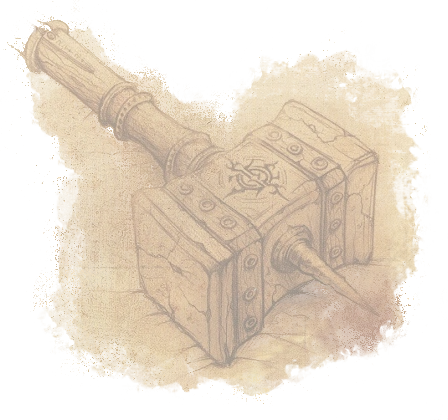
\includegraphics[width=1.3\columnwidth]{%
		images/Magic_Items/Hammer_of_Glory_background.png%
	}};%
\end{tikzpicture}%

\subsection*{Gameplay Mechanics}
{\entryfont The Staff of the Evoker holds a number of charges equal to the value listed for each state. It regains regains expended charges as specified daily at dawn.
\subsubsection*{Dormant State}
\textbf{Charges: 3, Recharge: 1d2 + 1}
\begin{itemize}
	\item The wielder gains a +1 bonus to attack and damage rolls made with this weapon.
	\item While holding the staff, the wielder can expend some of its charges to cast one of the following spells from it, using their spell save DC and spellcasting ability:
	\begin{itemize}
		\item Burning Hands (1 Charge)
		\item Melf's Acid Arrow (2 Charges)
	\end{itemize}
\end{itemize}
\paragraph*{Awaken}
\subsubsection*{Awakened State}
\textbf{Charges: 5, Recharge: 1d4 + 1}
\begin{itemize}
	\item The bonus to attack and damage rolls increases to a +2.
	\item The following spells to the list of spells the staff may be used to cast are added:
	\begin{itemize}
		\item Melf's Minute Meteor (3 Charges)
		\item Storm Sphere (4 Charges)
	\end{itemize}
\end{itemize}
\paragraph*{Exalt}
\subsubsection*{Exalted State}
\textbf{Charges: 7, Recharge: 1d6 + 1}
\begin{itemize}
	\item The bonus to attack and damage rolls increases to a +3.
	\item The following spells to the list of spells the staff may be used to cast are added:
	\begin{itemize}
		\item Maelstrom (5 Charges)
		\item Heal (6 Charges)
	\end{itemize}
	\item The wielder can use the \textbf{Bramble Shot} ability twice between rests, and the Saving Throw DC increases to 17.
\end{itemize}}